\section{$\mathbf{X} = \mathbf{U\Sigma V^T}$ Eigenanalysis, Singular Value Decomposition (SVD)}
\label{sec:datasvd}

Singular Value Decomposition (SVD) is a matrix decomposition of the form $\mathbf{A}=\mathbf{U}\Sigma\mathbf{V}^T$, where $\mathbf{U}$ and $\mathbf{V}$ are both unitary (cf. section \ref{sec:svd}). The decomposition always exists for a general complex matrix $\mathbf{A}\in\mathbb{C}^{m\times n}$. 
\\

If $\mathbf{X}\in\mathbb{R}^{N\times p}$ is a data matrix with $N$ samples in the rows and $p$ features in the columns, then SVD allows for the decomposition of the data into $p$ linearly independent components, ranked by their explained variance (i.e. their strength in the dataset). The basis of the decomposition turns out to be the same as for PCA (cf. section \ref{sec:pca}) except that it is arrived at slightly differently, because PCA involves diagonalizing the covariance matrix., nor are the singular values the same as the explained variances of the dataset. The decomposition of the dataset can be understood as follows. In the SVD of the data matrix: 

\begin{equation}
\mathbf{X} = \mathbf{U}\mathbf{\Sigma}\mathbf{V}^T
\end{equation}

The individual rows of $\mathbf{X}$, i.e. the individual data points, are expressed as:

\begin{equation}
\mathbf{x}^T_i = \sum_{j=1}^p u_{i,j}\sigma_j\mathbf{v}_j^T
\end{equation}

Where $\mathbf{x}_i$ is the $i$th data point. Hence the right singular vectors $\mathbf{v}_i$ are the normalized basis vectors, and the columns of $\mathbf{U}$ give the coefficients the basis expansion, together with the singular values $\sigma_i$, which give a measure of the global strength of the corresponding basis vector. 

Truncating the expansion after the $r$th term results in a rank $r$ approximation of $\mathbf{X}$ known as the \textit{truncated singular value decomposition} (TSVD) estimator. According to the Eckart-Young Mirsky-Theorem, the estimator is the best rank-$r$ approximation under the Frobenius norm of the error (cf. \ref{sec:frobenius}), which is the average mean square error across $\mathbf{X}$. 

\begin{equation}
\mathbf{\hat{X}} = \sum_{i=1}^r \sigma_i (\mathbf{u}_i \otimes \mathbf{v}_i)
\end{equation}

Since it minimizes the average mean square error, $\mathbf{\hat{X}}$ is the rank $r$ maximum likelihood approximation to $\mathbf{X}$ under the assumption of normally distributed noise. Optimal truncation is discussed in section \ref{sec:truncation}.

SVD is scalable to very large datasets and finds many applications in the wild, including page rank, facial recognition, recommendation algorithms, and others. Randomized SVD (cf. section \ref{sec:rsvd}) is an approximate method that gives an even faster speedup.


% eigenfaces
\subsection{Example: Eigenfaces and Facial Recognition}
One famous result are the so-called eigenfaces. The data matrix $\mathbf{X}\in\mathbb{R}^{N\times p}$ consists of $N$ pictures of faces that each have $p$ pixels. The right singular eigenvectors yield $p$ eigenfaces in terms of which any of the $N$ pictures can be expressed. 

Below are the first eigenfaces extracted from the "Labeled Faces in the Wild" dataset, which includes 13233 portraits with 62x47=2914 pixels each. Running SVD on the data matrix $\mathbf{X} \in \mathbb{R}^{13233\times 2914}$ yields the eigenfaces shown in Figure \ref{fig:svd_eigenfaces}.

\begin{figure}
\centering
    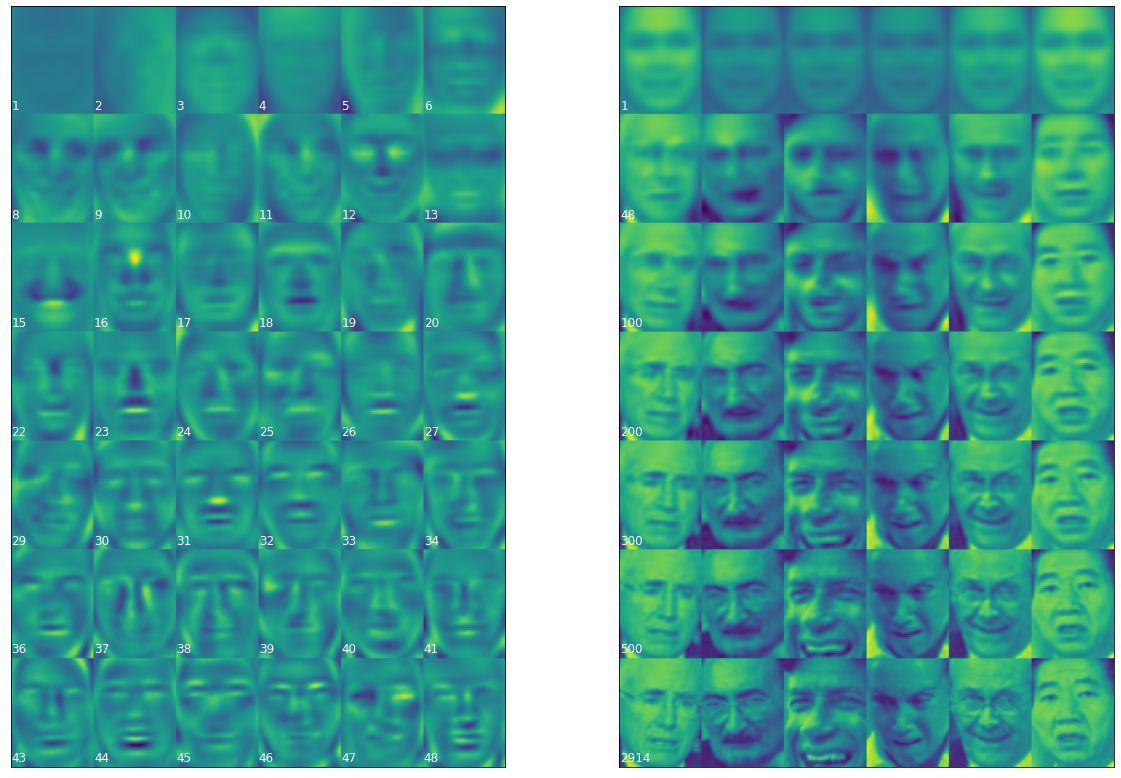
\includegraphics[width=\textwidth]{svd_eigenfaces.png}
    \caption{Left: The first 48 eigenfaces. The colorscale is consistent across the images. As can be expected, the eigenfaces seem to have an ordering from more general features, that are highly prevalent in the dataset, towards more specific features. Right: Five sample portraits from the dataset approximated using different numbers of eigenvectors. 2914 corresponds to the original image, which had 2914 pixels (degrees of freedom).}
    \label{fig:svd_eigenfaces}
\end{figure}

Facial recognition may be performed by projecting a new face into the space of eigenfaces and matching to the coefficients of a known subject. This could be done using the euclidean distance, or it could be done using a classifier. In case of classificiation, the dimensionality reduction that is enabled by approximating images with a smaller set of eigenvectors may be critical to making the problem tractable by overcoming the curse of dimensionality. When the data matrix is not centered (that is, the mean is not subtracted from it before performing the SVD), then the first right singular vector is vector close to the average row in the matrix.


% eigenbasis 
\subsection{Tracking an Eigensystem over Time}
\label{sec:svd_tracking}
	
As discussed in section \ref{sec:svd}, the sign of the basis vectors can be flipped without affecting the validity of the singular value decomposition. That means that if the SVD is performed on some system may equally well return, say, a left-handed or a right-handed coordinate system. This becomes a problem when the results of repeated SVDs are supposed to be compared, for example to study the evolution of a system over time. Figure \ref{fig:svd_consistently_oriented} shows the eigenbasis of a bivariate Gaussian with principal axes slowly rotating over a 180-degree angle. The top shows how the eigenbases that is found flips back and forth, so that there is a double-trajectory corresponding to results with positive and negative sign on an eigenvector. The trajectory is not described by an injective function, which complicates analysis. 


\subsubsection{Heuristic Method}
Say an SVD is performed on a slowly-evolving system at time $t=0$ and at time $t=1$. To compensate the sign flips, a heuristic method is to first match the basis vectors at $t=0$ to the basis vectors at $t=1$ using a distance metric that is immune to the sign of the vectors, for example the absolute value of the dot product. (This assumes that the vectors are similar enough at time $t=0$ and $t=1$ that the matching an be done unambiguously. For the higher-order singular vectors this might be a problem, because they have lower numerical certainty.) Once the vectors are matched, the sign of the inner product between the vectors at $t=0$ and $t=1$ may be compared, and the sign flipped accordingly. 

This method works, but the problem is that the sign of the vectors is somewhat arbitrarily pinned relative to the result at $t=0$. That is, if, for example, the coordinate system found at $t=0$ was left-handed, then the time series of eigenbases will be adjusted to be left-handed. If the point of comparison had instead been the SVD performed at some other time $t=t'$, then one might have wound up with a right-handed coordinate system instead. It is desirable to find a consistent orientation.   


\subsubsection{Consistent Method}

\citeasnoun{damask2019consistently} recently developed a method that can be used to find a consistently oriented basis. Consistent orientation in this case means, roughly, that the eigenbasis is always flipped to obey the convention of being right-handed. The method relies on reconstructing the rotations and reflections necessary to transform the eigenbasis in question to the natural basis $\mathbf{I}$ as reference. While rotations preserve the orientation of a basis, but reflections do not. When the reflections of an eigenbasis with respect to the natural basis are known, then they can be undone by flipping them back in place. 


\begin{figure}
\centering
    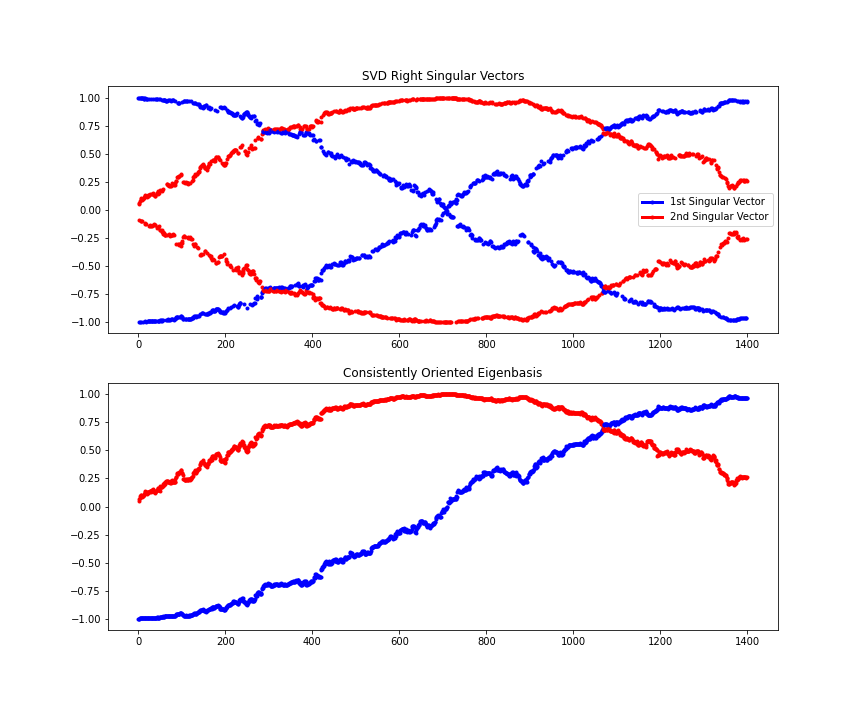
\includegraphics[width=\textwidth]{svd_consistently_oriented.png}
    \caption{Right singular vectors extracted using SVD, showing sign flips (top) and with a consistently oriented basis (bottom). The underlying data is a bivariate gaussian with principal axes undergoing a 180 degree rotation. With the consistently oriented basis, the singular vectors trace out a one-to-one trajectory that can be analyzed.}
    \label{fig:svd_consistently_oriented}
\end{figure}


\subsubsection{Rank Order Changes}

The singular vectors or eigenvectors of a system are labeled only in terms of their associated singular values or eigenvalues. In order to track a singular vector throughout rank order changes, it is necessary to figure out a way to attach a separate label, for example by looking at the "content" of a particular singular vector. How well that works has to be figured out in context, I am not currently aware of a generally valid solution. 


% Bayesian SVD
\subsection{Bayesian SVD}
To do! Cf. https://ieeexplore.ieee.org/document/7336426

It's awful to be tied to the assumption of normality and it's awful to not know the uncertainty of my singular vectors!






